\section{Thuật toán Zhu-Takaoka}

\subsection{Đặc điểm chính}
Thuật toán Zhu-Takaoka là một biến thể của thuật toán Boyer-Moore, được đề xuất bởi Rui Feng Zhu và Tadao Takaoka nhằm cải thiện hiệu quả của phép dịch chuyển bad-character. Khác với Boyer-Moore truyền thống chỉ xét một ký tự, thuật toán này sử dụng đồng thời hai ký tự liên tiếp của văn bản để tính toán khoảng dịch chuyển, từ đó có thể tạo ra các bước dịch chuyển lớn hơn trong nhiều trường hợp thực tế.

Nhờ khai thác thông tin từ cặp ký tự liên tiếp, Zhu-Takaoka thường đạt hiệu năng tốt hơn Boyer-Moore khi làm việc với bảng chữ cái nhỏ hoặc các mẫu có độ dài lớn.

Thuật toán có các đặc điểm sau:
\begin{itemize}
    \item là một biến thể của thuật toán Boyer-Moore;
    \item sử dụng hai ký tự liên tiếp của văn bản để tính phép dịch chuyển bad-character;
    \item giai đoạn tiền xử lý có độ phức tạp thời gian và không gian $O(m + \sigma ^ 2)$;
    \item giai đoạn tìm kiếm có độ phức tạp thời gian $O(mn)$.
\end{itemize}

\subsection{Mô tả thuật toán}
Zhu và Takaoka đã thiết kế một thuật toán thực hiện phép dịch chuyển bằng cách xét phép dịch chuyển bad-character cho hai ký tự liên tiếp của văn bản (xem thuật toán Boyer-Moore).

Trong giai đoạn tìm kiếm, các phép so sánh được thực hiện từ phải sang trái. Khi cửa sổ được đặt trên đoạn văn bản $y[j \dots j + m - 1]$ và xảy ra sự không khớp giữa $x[m - k]$ và $y[J + m - k]$, trong khi:

\[
x[m - k + 1 \dots m - 1] = y[j + m - k + 1 \dots j + m - 1],
\]

thì phép dịch chuyển được tính dựa trên hai ký tự văn bản $y[j + m - 2]$ và $y[j + m - 1]$. Bảng dịch chuyển good-suffix cũng được sử dụng để tính toán khoảng dịch chuyển.

Giai đoạn tiền xử lý của thuật toán bao gồm việc tính toán, với mỗi cặp ký tự $(a, b)$, trong đó $a, b \in \Sigma$, lần xuất hiện ngoài cùng bên phải của chuỗi $ab$ trong đoạn $x[0 \dots m - 2]$.

Với $a,b \in \Sigma$:

\[
ztBc[a,b] =
\begin{cases}
k, & \text{nếu } k < m-2,\ x[m-k \dots m-k+1] = ab \\
   & \text{và } ab \text{ không xuất hiện trong } x[m-k+2 \dots m-2]; \\

m-1, & \text{nếu } x[0] = b \\
     & \text{và } ab \text{ không xuất hiện trong } x[0 \dots m-2]; \\

m, & \text{nếu } x[0] \neq b \\
   & \text{và } ab \text{ không xuất hiện trong } x[0 \dots m-2].
\end{cases}
\]

Thuật toán cũng cần tính bảng $bmGs$ (xem thuật toán Boyer-Moore).

Giai đoạn tiền xử lý có độ phức tạp thời gian và không gian $O(m + \sigma ^ 2)$. Giai đoạn tìm kiếm có độ phức tạp thời gian bậc hai trong trường hợp xấu nhất.

\subsection{Cài đặt bằng C++}

\begin{verbatim}
#include <iostream>
#include <vector>
#include <string>
#include <algorithm>

using namespace std;

const int ASIZE = 256;

/* ---------- Suffixes ---------- */
void suffixes(const string &pat, vector<int> &suff) {
    int m = pat.length();

    suff.resize(m);
    suff[m - 1] = m;

    int g = m - 1;
    int f = 0;

    for (int i = m - 2; i >= 0; --i) {
        if (i > g && suff[i + m - 1 - f] < i - g) {
            suff[i] = suff[i + m - 1 - f];
        } else {
            if (i < g)
                g = i;

            f = i;

            while (g >= 0 &&
                   pat[g] == pat[g + m - 1 - f]) {
                --g;
            }

            suff[i] = f - g;
        }
    }
}

/* ---------- Good Suffix ---------- */
void preBmGs(const string &pat, vector<int> &bmGs) {
    int m = pat.length();

    vector<int> suff;
    suffixes(pat, suff);

    bmGs.assign(m, m);

    int j = 0;

    for (int i = m - 1; i >= 0; --i) {
        if (suff[i] == i + 1) {
            for (; j < m - 1 - i; ++j) {
                if (bmGs[j] == m)
                    bmGs[j] = m - 1 - i;
            }
        }
    }

    for (int i = 0; i <= m - 2; ++i) {
        bmGs[m - 1 - suff[i]] = m - 1 - i;
    }
}

/* ---------- Zhu-Takaoka Bad Character ---------- */
void preZtBc(const string &pat,
             vector<vector<int>> &ztBc) {
    int m = pat.length();

    ztBc.assign(ASIZE, vector<int>(ASIZE, m));

    for (int i = 0; i < ASIZE; ++i) {
        ztBc[i][(unsigned char)pat[0]] = m - 1;
    }

    for (int i = 1; i < m - 1; ++i) {
        ztBc[(unsigned char)pat[i - 1]]
             [(unsigned char)pat[i]]
            = m - 1 - i;
    }
}

/* ---------- Zhu-Takaoka Search ---------- */
void ZT(const string &pat, const string &txt) {
    int m = pat.length();
    int n = txt.length();

    vector<vector<int>> ztBc;
    vector<int> bmGs;

    /* Preprocessing */
    preZtBc(pat, ztBc);
    preBmGs(pat, bmGs);

    /* Searching */
    int j = 0;

    while (j <= n - m) {
        int i = m - 1;

        while (i >= 0 &&
               pat[i] == txt[i + j]) {
            --i;
        }

        if (i < 0) {
            cout << "Pattern found at index: "
                 << j << endl;

            j += bmGs[0];
        } else {
            j += max(
                bmGs[i],
                ztBc[(unsigned char)txt[j + m - 2]]
                     [(unsigned char)txt[j + m - 1]]
            );
        }
    }
}

/* ---------- Main ---------- */
int main() {
    string text = "ABAAABCDABCABC";
    string pattern = "ABC";

    ZT(pattern, text);

    return 0;
}
\end{verbatim}

\subsection{Kiểm nghiệm thuật toán}

\textbf{Pha tiền xử lý:}

\begin{figure}[H]
    \centering
    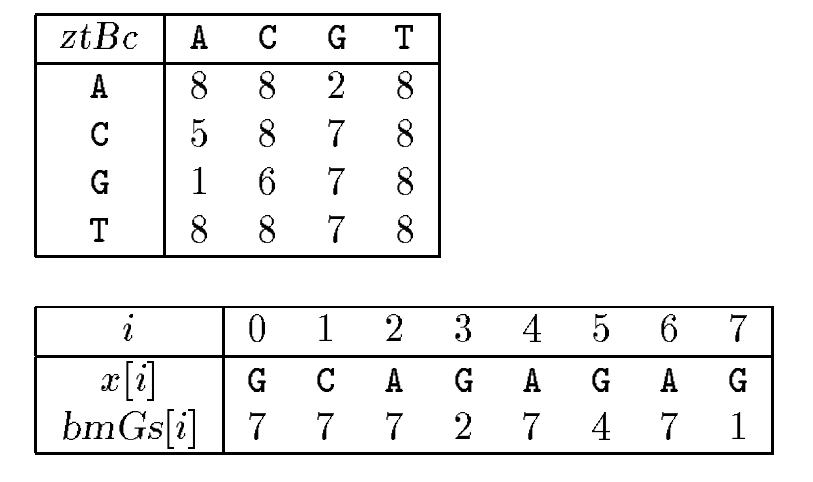
\includegraphics[width=15cm]{Images/2026-05-18-10-50-01.png}
    \caption{Kết quả tiền xử lý bảng ztBc và bmGs của thuật toán Zhu-Takaoka}
    \label{fig:zhu-takaoka-preprocess}
\end{figure}

Bảng $ztBc$ và $bmGs$ được sử dụng bởi thuật toán Zhu-Takaoka.

\textbf{Pha tìm kiếm:}

Lần 1:

\begin{figure}[H]
    \centering
    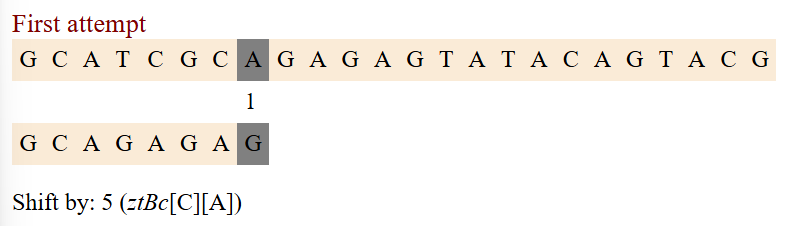
\includegraphics[width=15cm]{Images/2026-05-18-10-50-57.png}
    \caption{Bước 1 trong quá trình thực hiện thuật toán Zhu-Takaoka}
    \label{fig:zhu-takaoka-step-1}
\end{figure}

Lần 2: 

\begin{figure}[H]
    \centering
    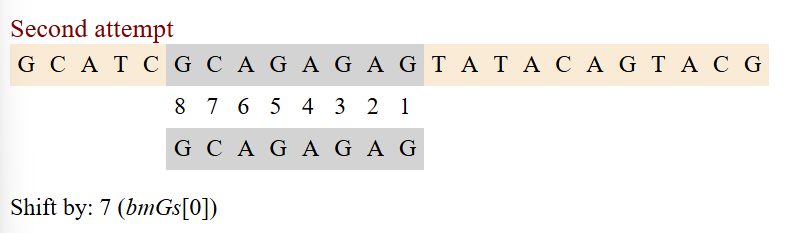
\includegraphics[width=15cm]{Images/2026-05-18-10-51-18.png}
    \caption{Bước 2 trong quá trình thực hiện thuật toán Zhu-Takaoka}
    \label{fig:zhu-takaoka-step-2}
\end{figure}

Lần 3:

\begin{figure}[H]
    \centering
    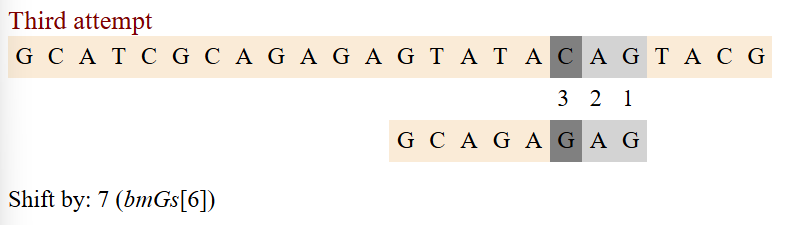
\includegraphics[width=15cm]{Images/2026-05-18-10-51-33.png}
    \caption{Bước 3 trong quá trình thực hiện thuật toán Zhu-Takaoka}
    \label{fig:zhu-takaoka-step-3}
\end{figure}

Thuật toán Zhu-Takaoka thực hiện 12 phép so sánh ký tự trong ví dụ trên.

